\chapter{Introduction}
\section{Motivation}
Software defect prediction(SDP) is kind of technique for software checking and the debugging. It will cost much for a software maintenance at later period. Since,By using SDP, the developers can focus on the modules that most likely have bug.\\
\\
Recent technique mainly base on machine learning model to predict the whether a file or a bug have bug or not. this method mainly make use of history data, then construct a series of metrics to train the model, so that it can be utilized to predict the buggy of other modules.\\

Since building a effective metric is essential in a machine learning model, many researcher have proposed their concept and idea to construct the metric of SDP model, in the early research, Line Of Code (LOC)\cite{} was employed to measure if file that have bug or not. However, such simple metric ignores the structure of code. Halstead proposed a software complexity metric by counting the occurrence of operator and operand in the source code \cite{}. McCabe also raise concept of cyclomatic complexity that possibility of causing bugs increase as the program becomes more complex\cite{}. CK metrics suit measures the software complexity by considering its inheritance, coupling, and cohesion. MOOD \cite{} metrics are also be proved as effective in SDP. \\

As for machine learning model, many classical machine learning model are adopted for SDP. such as logistics regression (LR), support vector machine (SVM),decision tree (DT), random forest (RF), Adaboost, and naive bayes (NB). Moreover, ensemble learning strategy such as voting, stacking and averaging are perform well in SDP. 

However, traditional machine learning base model may have some problem:
\begin{itemize}
    \item Need to construct metric manually.
    \item Do not consider the semantics of code.
\end{itemize}

Traditional machine learning model need to extract features manually to construct a machine learning model. Thereby, the quality of feature is directly impact the performance of machine learning model. Besides, traditional metrics did not consider the semantics of programs. Take Figure 1.1 as example, \texttt{foo()} function and \texttt{bar()} fucntion has the same of count of line of code. When we select \texttt{add()} and \texttt{remove()} as the information node of these two code snippets, we will generate [\texttt{add(0)},\texttt{remove(0)},\texttt{remove(0)},\texttt{add(0)}] and [\texttt{add(0)},\texttt{remove(0)},\texttt{add(0)},
\texttt{remove(0)}] for \texttt{foo()} and \texttt{bar()},respectively. However, \texttt{foo()} will occur exception. Traditional metrics can not identify such feature, so called semantics features. To solve this problem. Wong et.al \cite{} extract abstract syntax tree (AST) and select specific node from AST to present the code semantics, then they leverage word embedding technique to embed word into vectors and Finally employed deep belief network (DBN) \cite{} to extract feature from the embeded AST nodes and achieved better performance than traditional models. Song et.al also adopted Convolutional Neural Networks (CNN) to extract the features of programs, which also perform better than traditional machine learning model. Tree-base LSTM was employed to solve different level semantics of programs.\\

\begin{figure}
    \centering
    \subfigure[]{
    \begin{minipage}[t]{0.48\linewidth}
    \centering
    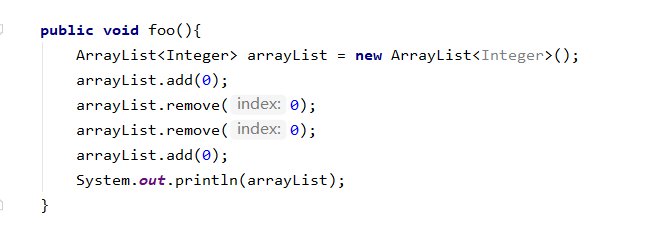
\includegraphics[width=3in]{pic/foo.png}
    \end{minipage}
    }
    \subfigure[]{
    \begin{minipage}[t]{0.48\linewidth}
    \centering
    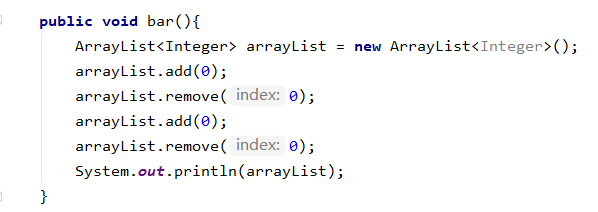
\includegraphics[width=3in]{pic/bar.png}
    \end{minipage}
    }
    \caption{a motivation example}
\end{figure}

Undoubly, such existing deep learning model can effective improve the performance of SDP, however, they still have some problems 
\begin{itemize}
    \item Limited by training data, the token may not be trained sufficiently.
    \item Not be able to learn identical tokens semantics in different context
\end{itemize}

Limited by existing public defect dataset, the number of instance in the largest project is no more than 2000, thereby tokens may not be trained sufficiently in token embedding phrase. Besides, it can also llanguage model. Different from \textit{Word2vec} model, the \textit{BERT} model can learn the ead to overfiting problem when deep learning model constructed with large count parameter. To solve this problem, we proposed data augmentaion strategy to generate more data for training. To ensure that token can be well-trained, we pretrain large Java source code using  \textit{BERT} semantics of identical token under different semantics. \\

On the one hand, tokens in training data not appeared in test data which will impact the performance of model.On the other hand, existing researches mainly select specific nodes from ASTs tree and generate sequence. Though, such kind of approaches can learn the semantics of source code, whereas it ignore large kind node. The result is that vocabulary size become smaller compare with the approach that use all tokens from source code. \\ 

Since attention based LSTM and CNN are show excellent performance in text classification and previous, we make use of both ability to learn the semantics to generate features. BiLSTM can learn context information in a sequence while attention mechnism can foucs the token with important information. CNN can learn the local information of sequence. Both two approach are widely applied in academic research and industry.

Base on the problem that given above, we raise several research questions to validate the effectiveness of our model.\\

\textbf{RQ1:Can data augmentation improve the performance of our model?}. To verify our assumption that more data for training can improve the performance, we conducted the experiment by boosting training dataset. 

\textbf{RQ2: Can our model outperform other models including traditional metrics based models and deep learning based models?}. To verify whether our model are better than existing deep learning model, we select to deep learning models, CNN model as baseline to compare with our model. For traditional features base model, we construct two baseline with logistics regression as traditional model.

\textbf{RQ3: Is BERT prtreained model Better than Word2vec pretrained model}. We investigate which kind of information are better for SDP.

\textbf{RQ4: Which data preprocessing method is better for Software defect prediction?}. Since mainly researches parse source code into ASTs while another is make use all the tokens. We compare both two preprocessing method to investigate which form is better for SDP.

The rest part of this paper is follows. Chapter 2 introduce the relevant researches and background; chapter 3 introduces the details of proposed model; chapter 4 ilustrate how we design the experiments for research questions; chapter 5 is the results of our experiments; chapter 6 is discussion of our results; chapter 7 is the conclusion of our experiments.





